\documentclass[class=scrartcl]{standalone}
\usepackage{chez}

\begin{document}
If we have the control flow graph,
we can define a function that gives
what is true at the beginning of each block,
and at the end of each block.
When two paths meet, we can take the meet \((\wedge)\)
of the invariants that are true.
We can then solve this through \vocab{chaotic iteration}:
\begin{itemize}[nosep]
  \item Keep a list of nodes to update.
  \item Pick one of the control flow graph nodes.
  \item Update the exit invariant for this node.
  \item If the exit invariant is updated,
        add the children to a queue to visit next.
\end{itemize}

\section{Collecting Semantics}
We are interested in the states that a program may be in at a given point.
In particular, if we have a program with labeled points,
we want to find a function
\[
  \mathcal C \colon \text{Labels} \to \mathcal P(\Sigma).
\]
\begin{center}
  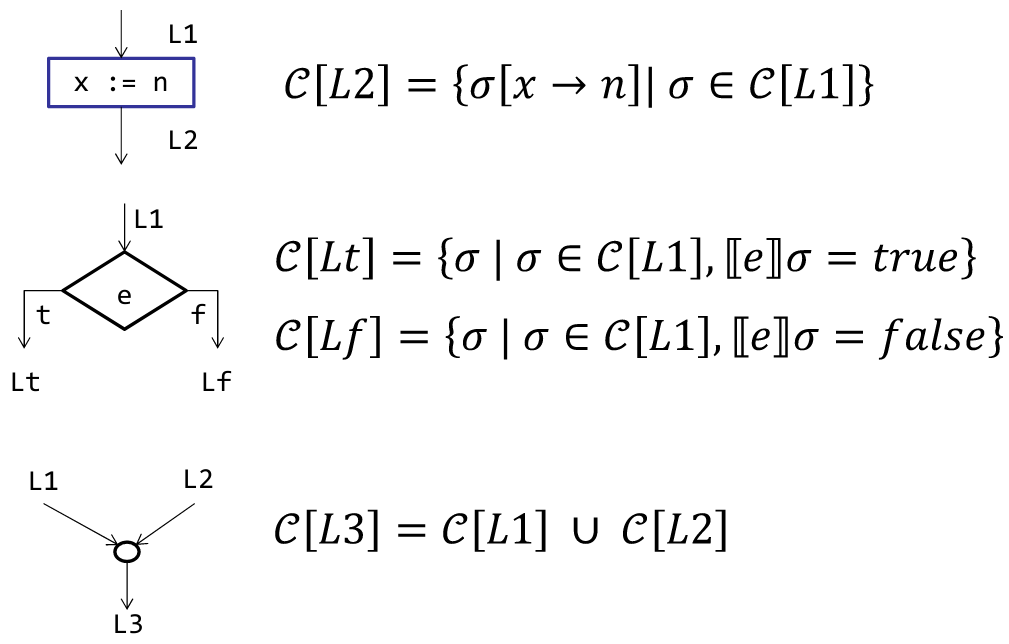
\includegraphics[width=0.5\textwidth]{collecting-semantics.png}
\end{center}

Note that before, we analyzed programs based on the syntax,
but here, we're looking at the control flow graph.

Like computing weakest preconditions,
computing the collecting semantics is undecidable,
but we can compute an approximation
\(\mathcal A \colon \text{Labels} \to \mathcal P(\Sigma)\),
which is sound as long as \(\mathcal C[L_i] \subseteq \mathcal A[L_i]\).

To do this, we define an \vocab{abstraction domain},
which is a lattice of abstract program states.
Then, we have two functions:
\begin{itemize}[nosep]
  \item \vocab{Abstraction function}
        \(\alpha \colon \mathcal P(\mathcal V) \to \text{Abs}\)
        that maps a value in the program to the ``best'' abstract value.
  \item \vocab{Concretization function}
        \(\gamma \colon \text{Abs} \to \mathcal P(\mathcal V)\),
        mapping an abstract value to a set of possible states.
\end{itemize}
These functions satisfy the identity
\[
  \forall a \in \text{Abs},
    \forall V \in \mathcal P(\mathcal V),
      V \subseteq \gamma(a) \iff \alpha(V) \leq a.
\]
This is called the \vocab{Galois connection}, which comes from algebra.
Note that both functions are monotonic, i.e.
\begin{gather*}
  V \subseteq V' \implies \alpha(V) \leq \alpha(V') \\
  a \leq a' \implies \gamma(a) \subseteq \gamma(a').
\end{gather*}
This implies \(\alpha(\gamma(a)) \leq a\).


Now suppose we have some operator \(\diamond\).
We can define
\[
  \diamond \colon \text{Abs} \times \text{Abs} \to \text{Abs}
\]
by lifting the operation with
\[
  a_1 \diamond a_2 = \alpha(\gamma(a_1) \diamond \gamma(a_2)),
\]
where \(\diamond\) on the right takes all possible combinations.
Then we have
\[
  \gamma(a_1 \diamond a_2) \supseteq \gamma(a_1) \diamond \gamma(a_2),
\]
since the abstraction \(a_1 \diamond a_2\) may lose information.

In general, we must define the abstraction domain,
abstraction and concretization function,
and also the transfer function,
which describes how the functions interact with operators.

\begin{example}[Constant domain]
  Consider the lattice \(\set{\top, \bot} \union \ZZ\)
  where \(\bot \leq n\) and \(n \leq \top\) for all \(n \in \ZZ\).
  \TODO[draw picture]
  
  Suppose our program has states of the form \(\parens{x = k, y = \ell}\)
  where \(k, \ell \in \ZZ\).
  Then we can define the concretization function
  \[
    \gamma(\set{x = a_x, y = a_y}) =
      \set{(x, y) \mid x \in \gamma'(a_x),
                       y \in \gamma'(a_y)}
  \qquad \text{where} \qquad
    \gamma' = \begin{cases}
      \top \to \ZZ \\[-1ex]
      \bot \to \nullset \\[-1ex]
      n \to \set{n}
    \end{cases}
  \]


\end{example}




\end{document}
